% !TeX spellcheck = ru_RU
%pdflatex, utf8
\documentclass[unicode, 10pt, a5paper, oneside]{article}

% Установка полей страницы
%\usepackage{anysize}
%\marginsize{0.3cm}{0.3cm}{0.3cm}{0.3cm}
\usepackage[a5paper, margin=0.3cm, bindingoffset=0cm]{geometry}

% Поддержка русского языка
\usepackage[T2A]{fontenc}		% Корректная кодировка шрифта при использовании cm-super
\usepackage[utf8]{inputenc}		% Кодировка ввода
\usepackage[russian]{babel}		% Словарь расстановки переносов
%\usepackage{cmap}				% Перекодировка символов в pdf при использовании обычного cm

% Всякие математические фишки
\usepackage{amsmath}
\usepackage{amsfonts}
\usepackage{amssymb}

% Изменение цвета, работа с графикой
\usepackage{color}
\usepackage[pdftex]{graphicx}
\graphicspath{{images/}}

% Команда для вставки ссылок \url{URL}
\usepackage[hyphens]{url}
\urlstyle{rm}					% Стиль шрифта ссылок: с засечками

% Кликабельные ссылки внутри документа
\usepackage[unicode]{hyperref}

% Включает отступ у первого абзаца в разделе
\usepackage{indentfirst}

% Настрйока стиля списков
\usepackage{enumitem}
\setlist{noitemsep, leftmargin=*, labelindent=\parindent, topsep=0pt, parsep=0pt, partopsep=0pt}

\setlist[itemize,1]{label=$\diamond$}
\setlist[itemize,2]{label=\textendash}
\setlist[itemize,3]{label=$\star$}

\renewcommand{\alph}[1]{\asbuk{#1}} % Костыль для кирилической нумерации вместо латинской
\setlist[enumerate,1]{label=\arabic*)}
\setlist[enumerate,2]{label=\alph*)}
\setlist[enumerate,3]{label=(\arabic*)}


\usepackage{textcomp}			% Команды для вставки разных символов (градусы, проценты, итд)
\usepackage{float}				% Размещение плавающих объектов там где они созданы (X)
\usepackage{wrapfig}			% Обтекаемые текстом рисунки

% Подписи у флоатов
\setlength{\intextsep}{0pt} % Отстут вокруг плавающих окружений
\usepackage{caption}
\captionsetup{parskip=0pt}
\captionsetup[figure]{labelsep=period,justification=centering,singlelinecheck=false,textfont=small,labelfont=small,aboveskip=2pt,belowskip=0pt}

% Изменение формата заголовков разделов
\usepackage{titlesec}
\titleformat{\section}{\newpage\small\bfseries}{\thesection. }{0pt}{}{}
\titlespacing*{\section}{0pt}{0pt}{0pt}

\titleformat{\subsection}{\small\bfseries}{\thesubsection. }{0pt}{}{}
\titlespacing*{\subsection}{0pt}{0pt}{0pt}

\usepackage{array}				% Позволяет объявить свои типы колонок
\usepackage{calc}				% Математика, исп-ся для расчёта ширины колонки
\usepackage{longtable}			% Длинные таблицы

% Минимальный отступ в таблицах
\setlength{\tabcolsep}{1.5mm}

% Новые типы колонок. Ширина задётся как доля от linewidth
\newcolumntype{L}[1]{p{#1\linewidth-2\tabcolsep-2\arrayrulewidth}}
\newcolumntype{C}[1]{>{\centering}p{#1\linewidth-2\tabcolsep-2\arrayrulewidth}}
\newcolumntype{R}[1]{>{\raggedleft}p{#1\linewidth-2\tabcolsep-2\arrayrulewidth}}
\newcolumntype{U}[2]{p{#1\linewidth-(#2)}}

% Стараться не оставлять одиноких строк в начале и конце абзаца
\clubpenalty=1000
\widowpenalty=1000

% Расстановка отступов и переносов
\emergencystretch=2.5em			% Максимальный промежуток между словами
\tolerance=2000
\frenchspacing


\begin{document}

\setcounter{section}{140}

% Вопрос 141 --------------------------------------------------------
\section{Схемы мультивибратора на транзисторах и ОУ.}

Мультивибратор --- генератор колебаний прямоугольной формы с короткими фронтами. Мультивибратор работает в автоколебательном режиме и не имеет устойчивых состояний. По сути представляет собой двухкаскадный резистивный усилитель с глубокой положительной обратной связью. Длительность периода из двух частей равна:

\begin{displaymath}
T = t_1 + t_2 = \ln 2 \cdot R_2 C_1 + \ln 2 \cdot R_3 C_2
\end{displaymath}
\begin{figure}[H]
\centering
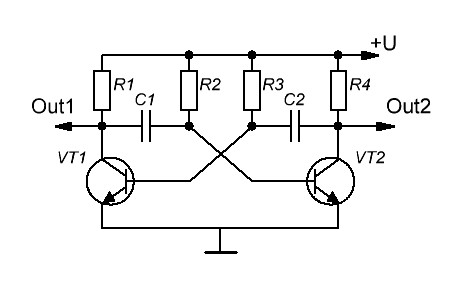
\includegraphics[width=0.4\textwidth]{141_tranz.jpg}
\caption{Мультивибратор на транзисторах}
\end{figure}
На ОУ строят мультивибраторы работающие на относительно низких частотах. Для регулировки соотношения длительности положительных и отрицательных импульсов применяется следующая схема (см. рис.).
\begin{figure}[H]
\centering
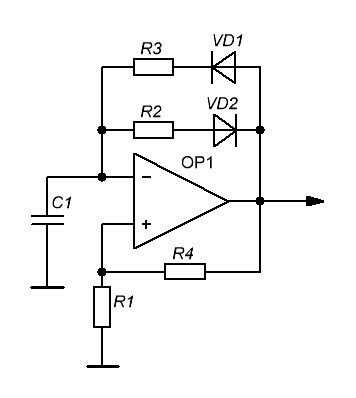
\includegraphics[width=0.35\textwidth]{141_OU_unsim.jpg}
\caption{Несимметричный мультивибратор на ОУ}
\end{figure}

Время импульса и паузы соответственно:
\begin{displaymath}
t_\text{и} = R_1 C_1 \ln (1 + 2 \frac{R_4}{R_3} )
\end{displaymath}
\begin{displaymath}
t_\text{п} = R_2 C_1 \ln (1 + 2 \frac{R_4}{R_3} )
\end{displaymath}
% Вопрос 142 --------------------------------------------------------
\section{Схема одновибратора на транзисторах.}

Одновибратор --- предназначен для формирования прямоугольных импульсов заданной длительности. Имеет одно устойчивое состояние, при котором VT1 закрыт, а VT2 открыт. Длительность генерируемого импульса $T_\text{имп} = 0,7 C_1 R_2 $.

\begin{figure}[H]
\centering
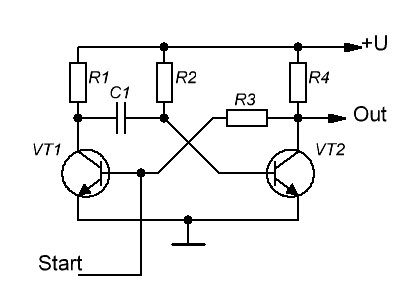
\includegraphics[width=0.4\textwidth]{142.jpg}
\caption{Одновибратор на транзисторах}
\end{figure}

% Вопрос 143 --------------------------------------------------------
\section{Масштабный усилитель на ОУ с К=+10.}

Так как коэффициент усиления положительный, усилитель неинвертирующий:
\begin{figure}[H]
\centering
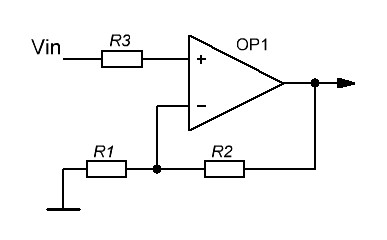
\includegraphics[width=0.4\textwidth]{143.jpg}
\caption{Масштабный усилитель}
\end{figure}
Коэффициент усиления вычисляется по формуле $K = 1 + \frac{R_2}{R_1} $. Отсюда, для получения коэффициента усиления 10 необходимо, чтобы выполнялось условие $R_2 = (K --- 1) R_1 = 9 R_1$. Выбор номиналов зависит от напряжения питания и требуемых токов. Резистор R3, устанавливаемый при необходимости, уменьшает ошибку, возникающую из-за тока смещения, и имеет номинал, равный $R_1 \parallel R_2$.

% Вопрос 144 --------------------------------------------------------
\section{Повторитель на ОУ.}
Рисовать смысла не имеет --- просто ОУ со 100\% отрицательной обратной связью. Сигнал поступает на неинвертирующий вход, снимается с выхода. Выходное напряжение равно напряжению на входе, входное сопротивление от 1 MОм до 10 TОм. Повторитель применяется как буферный усилитель, для исключения влияния низкоомной нагрузки на источник с высоким выходным сопротивлением.

% Вопрос 145 --------------------------------------------------------
\section{Двухтактный трансформаторный усилитель мощности, работающий в режиме АВ.}
Транзисторы работают поочередно, каждый во время своего полупериода входного двухполярного сигнала. Для перевода усилителя в режим АВ используются резисторы R1 и R2, создающие напряжение смещения на базах транзисторов (если бы их не было, то были бы искажения типа "ступенька", из-за использования нелинейной части характеристики транзисторов --- усилитель работал бы в режиме В).
\begin{figure}[H]
\centering
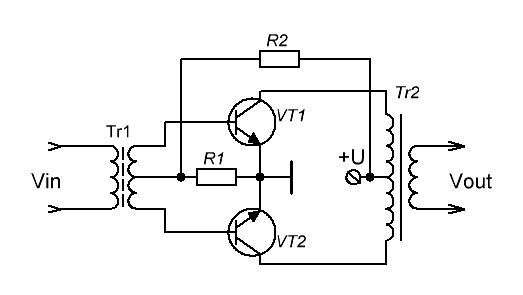
\includegraphics[width=0.6\textwidth]{145.jpg}
\caption{Двухтактный усилитель мощности}
\end{figure}

% Вопрос 146 --------------------------------------------------------
\section{Избирательные усилители LC и RC.}

Избирательные усилители предназначены для усиления сигналов в узкой полосе частот. По принципу действия различают усилители резонансные и с обратной связью. В резонансных в качестве нагрузки используется колебательный контур, имеющий большое сопротивление на резонансной частоте и малое на остальных. Избирательные свойства оцениваются добротностью $Q = \frac{f_0}{2 \Delta f}$, где $2 \Delta f$ --- полоса пропускания.
Усилители с ОС обычно используются на низких частотах. Резонансная частота такого усилителя определяется по формуле $f_0 = \frac{1}{2 \pi R C}$.
\begin{figure}[H]
\centering
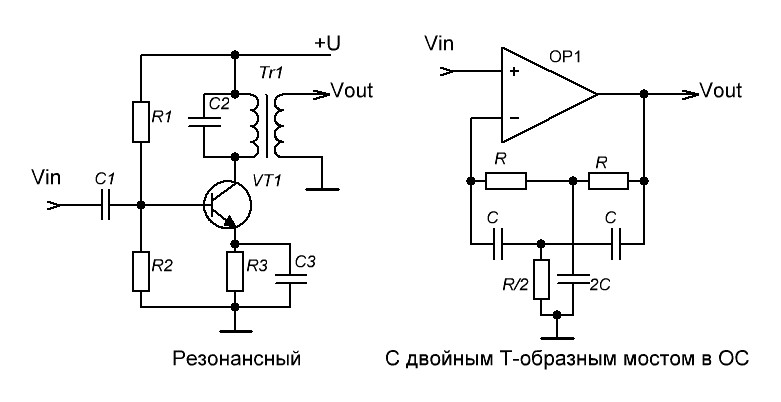
\includegraphics[width=0.7\textwidth]{146.jpg}
\caption{Избирательные усилители}
\end{figure}

% Вопрос 147 --------------------------------------------------------
\section{Схема стабилизатора напряжения на 10 В, 2 А на ИС К142.}

Микросхема К142ЕН3 (А, Б) представляет собой регулируемый стабилизатор напряжения с системой защиты от перегрева и перегрузки по току. При срабатывании системы защиты от перегрузки по току, выходное напряжение уменьшается почти до нуля. В случае срабатывания системы тепловой защиты, повторное включение стабилизатора возможно только после остывания микросхемы.

\begin{figure}[H]
\centering
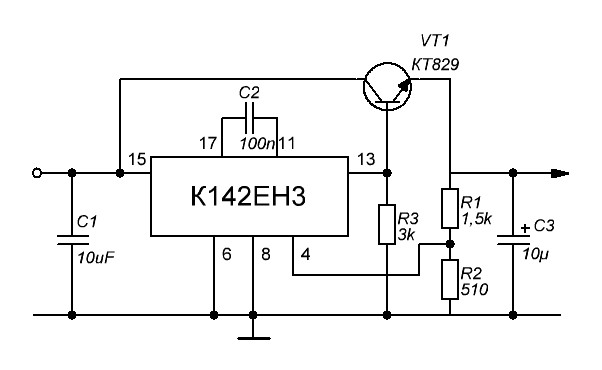
\includegraphics[width=0.6\textwidth]{147.jpg}
\caption{Стабилизатор на 10В, 2А}
\end{figure}

% Вопрос 148 --------------------------------------------------------
\section{Схема стабилизатора напряжения на 12 В, 1 А на ИС К142.}

Требуемым параметрам удовлетворяет микросхема К142ЕН8Б --- фиксированное напряжение стабилизации 12 В, ток до 1,5 А.
\begin{figure}[H]
\centering
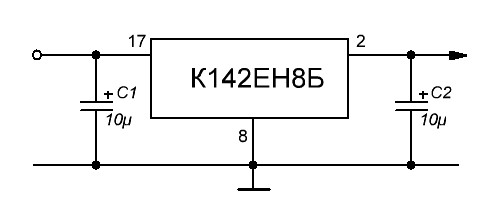
\includegraphics[width=0.55\textwidth]{148.jpg}
\caption{Стабилизатор на 12В, 1А}
\end{figure}

% Вопрос 149 --------------------------------------------------------
\section{Схема ключевого стабилизатора напряжения.}

Ключевые стабилизаторы напряжения обеспечивают значительно больший КПД за счет того, что транзистор работает в ключевом режиме, то есть потребляет только в открытом состоянии. При этом уменьшаются массогабаритные параметры стабилизатора. Однако, такие стабилизаторы могут стать причиной появления импульсных помех.

Ключевые стабилизаторы содержат накопительную индуктивность, включенную последовательно с нагрузкой. Для сглаживания пульсаций параллельно нагрузке стоит конденсатор. Ключ стоит между источником питания и накопительной индуктивностью. Устройство управления открывает/закрывает ключ в зависимости от напряжения на нагрузке.

При открытом состоянии транзистора напряжение поступает на выход, и одновременно энергия запасается в индуктивности. При отключении транзистора в нагрузке течет ток за счет самоиндукции индуктивности.

\begin{figure}[H]
\centering
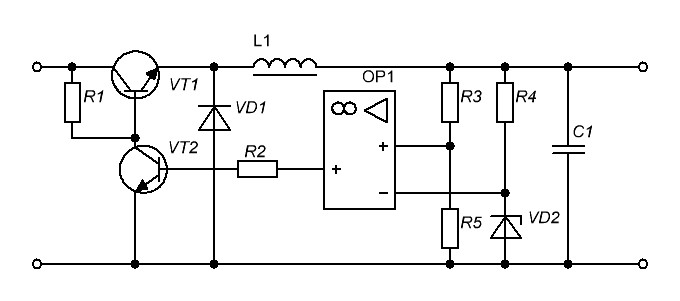
\includegraphics[width=0.7\textwidth]{149.jpg}
\caption{Ключевой стабилизатор}
\end{figure}

% Вопрос 150 --------------------------------------------------------
\section{Генератор гармонических колебаний на транзисторах.}

Генераторы гармонических колебаний строятся на основе усилителей с ПОС, обеспечивающих режим самовозбуждения на требуемой частоте. Для работы генератора необходимо выполнение условий баланса амплитуд и баланса фаз.

Генератор LC-типа предназначен для работы в диапазоне десятков кГц и более. Условия генерации здесь создаются на частоте резонанса:
\begin{displaymath}
f_0 = \frac{1}{2 \pi \sqrt{L C}}
\end{displaymath}

Фазовый сдвиг создается соответствующим подключением вторичной обмотки трансформатора. Баланс амплитуд достигается подачей соответствующей амплитуды сигнала с коллекторной нагрузки в цепь базы.

\begin{figure}[H]
\centering
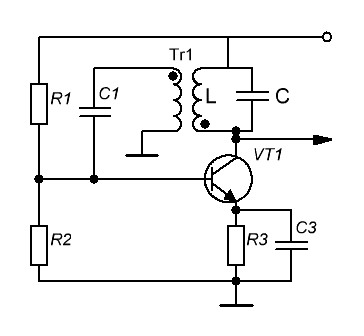
\includegraphics[width=0.45\textwidth]{150_lc.jpg}
\caption{LC-генератор}
\end{figure}

Кроме рассмотренной схемы, широкое распространение получили трехточечные схемы.

\begin{figure}[H]
\centering
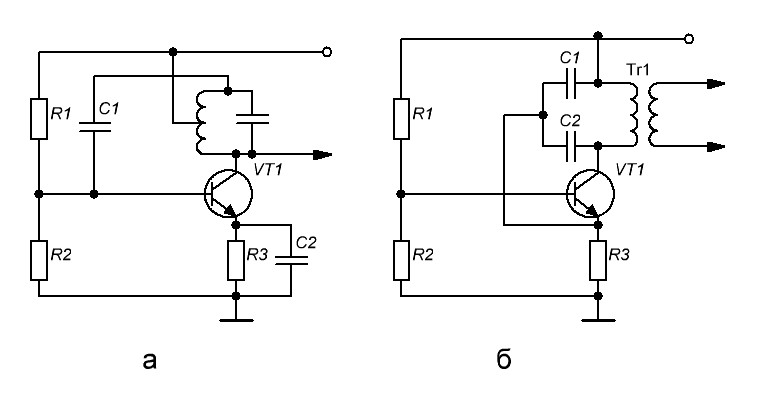
\includegraphics[width=0.55\textwidth]{150_3dot.jpg}
\caption{Трехточечные схемы с индуктивной автотрансформаторной (а) и емкостной (б) обратными связями}
\end{figure}

Генератор RC-типа --- резистивный усилитель, охваченный ПОС. Для получения фазового сдвига применяются фазовращающие цепочки с несколькими RC-звеньями (минимум 3). Обеспечение условий генерации выполняется подбором элементов в цепи ОС и инверсивными свойствами усилителя.

\begin{figure}[H]
\centering
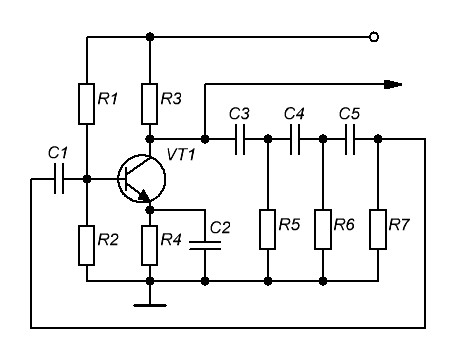
\includegraphics[width=0.5\textwidth]{150_rc.jpg}
\caption{RC-генератор}
\end{figure}

\end{document}